\documentclass[hyperref={pdfpagelabels=false}]{beamer}
\usepackage{graphicx,lmodern,subfigure,ulem,color,graphicx,tikz,booktabs}
\usetheme{default}
%\usecolortheme{seahorse}
\definecolor{beamer@blendedblue}{rgb}{0.1,0.5,0.1}
\definecolor{ForestGreen}{RGB}{60, 140, 60}
\setbeamercolor{structure}{fg=beamer@blendedblue}
\setbeamertemplate{navigation symbols}{}
\setbeamertemplate{footline}[frame number]

\usepackage{lmodern}
\newcommand{\spitem}{\vspace{.3cm}\item}

%commands
\newcommand{\elas}{$E_{labor}$}

\title[Capital Structure]{How labor market frictions affect capital structure\\ } 
\author[\insertframenumber/\inserttotalframenumber \hskip 1in 
]{Yasser Boualam, Marco Brianti, Tzuo Hann Law
}
\institute{UNC, BC, BC}

\date{\today}

\begin{document}
\frame{\titlepage \begin{center} Midwest Macro, Pittsburgh, 2017 \end{center} }


\frame{\frametitle{How does labor market frictions affect capital structure?}
\begin{figure}
	\centering
	\begin{itemize}
		\item Modigliani Miller 1958
		\item[] \textbf{Why does capital structure matter at all?}
		\item[] Bankruptcy costs can be high(er) after accounting for stakeholders who might not be (fully) represented at the bargaining table. 
		\item A firm's labor force is one such under-represented entity.
		\item \textbf{This paper:} How does adding capital structure to a workhorse labor market search model affect capital structure decisions?
	\end{itemize}
\end{figure}
}

\frame{\frametitle{What we do}
	\begin{figure}
		\centering
		\begin{itemize}
			\item Highlight empirical findings in the literature that call for the models we present.
			\item Present a simple three period model to highlight the channels.
			\item Present a fully dynamic model and do something...
		\end{itemize}
	\end{figure}
}


\frame{\frametitle{Main channels}
	\begin{figure}
		\centering
		\begin{itemize}
			\item Absent any search frictions, owners of production utilize optimal quantities of debt.
			\item With labor market frictions, the firm partners with a risk averse worker who potentially has the option to quit the partnership.
			\item While this quitting in a partial equilibrium setting benefits workers ex-post, it leads to less entry, less-than-optimal debt use, lower equilibrium wages and ex-ante lower value to workers.
		\end{itemize}
	\end{figure}
}

\frame{\frametitle{Literature}
	\begin{figure}
		\centering
		\begin{itemize}
			\item 
			\item
			\item
		\end{itemize}
	\end{figure}
}

\frame{\frametitle{Empirical observations}
	\begin{figure}
		\centering
		\begin{itemize} 
			\item
			\item
			\item
		\end{itemize}
	\end{figure}
}

\frame{\frametitle{Model without Labor Market Frictions}
	\begin{figure}
		\centering
		\begin{itemize}
			\item Debt is riskless. Borrows pay interest rate $ r $ and return all borrowed capital.
			\item A single agent with initial wealth chooses debt to maximize payoffs in two periods. The output in the first period must be weakly positive.
			\item[] \[\max_{D} \mathbb{E}u(c_1) + \beta \mathbb{E}u(c_2)\]
			\item where \[c_t(\phi_t) = \phi_t(W + D)^\gamma - rD\] is some decreasing returns production function with period productivity realization $ \phi \in U[0,1]$ and $ c_2  = 0 $ if $ c_1 < 0 $.
		\end{itemize}
	\end{figure}
}

\frame{\frametitle{Model without Labor Market Frictions: Solution}
	\begin{figure}
		\centering
		\begin{itemize}
			\item In this setup the optimal choice for debt $ D $ is
			\[ads\] 
			where we how the incompleteness of markets drives a wedge in the typical solution for equation the expected return of capital to the interest rate $ r $.
			\item Finally, note here that the owner of the firm can be the worker or the firm in a setting with both agents. 
		\end{itemize}
	\end{figure}
}

\frame{\frametitle{Labor Market Frictions with Capital Structure}
	\begin{figure}
		\centering
		\begin{itemize}
			\item Mortensen and Pissarides style search frictions.  
			\item Entrepreneurs own initial wealth $ W $ and borrow at rate $ r $. Debt is riskless.
			\item Debt choice is made before entry. No new debt or equity.
			\item Wage contracts are specified by \textit{unconstrained wages}, $ \tilde{w} $.
			\item $ \tilde{w} $ is restricted to be identical in both periods.
			\item Perfect commitment assumed. 
			\item No storage technology. 
		\end{itemize}
	\end{figure}
}

\frame{\frametitle{Timing}
	\begin{figure}
		\centering
		\begin{enumerate}
			\item \textbf{Period 0.} Firms with wealth, $ W $ choose debt $ D $ and enter.
			\begin{itemize}
				\item All workers are unemployed.
				\item Firm's post wage contracts, matching occurs.
				\item Unmatched firms exit immediately.
			\end{itemize}
			\item \textbf{Period 1.} Draw roductivity $ \phi $.
			\begin{itemize}
				\item If output is weakly negative, match is broken. Firm exits.
				\item Production + consumption occurs.
				\item Unmatched workers consume $ b $.
			\end{itemize}
			\item \textbf{Period 2.} Draw roductivity $ \phi $.
			\begin{itemize}
				\item Separation if output is below $ b $. 
				\item Production + consumption occurs. 
				\item Unmatched workers consume $ b $.
			\end{itemize}
		\end{enumerate}
	\end{figure}
}

\frame{\frametitle{Period production}
	\begin{figure}
		\centering
		\begin{itemize}
			\item Period output is given by
			\item[] \[\phi_t (W - COE - D)^\gamma - Dr\]
			\item If period output is negative, exit occurs.
			\item If output exceeds $ \tilde{w} $, workers are paid $ \tilde{w} $. 
			\item Dividends are positive iff $ (W - COE - D)^\gamma - Dr \ge w^* $
			\item Don't worry, we have pictures.
		\end{itemize}
	\end{figure}	
}

\frame{\frametitle{Period 1 Wages}
\begin{figure}
	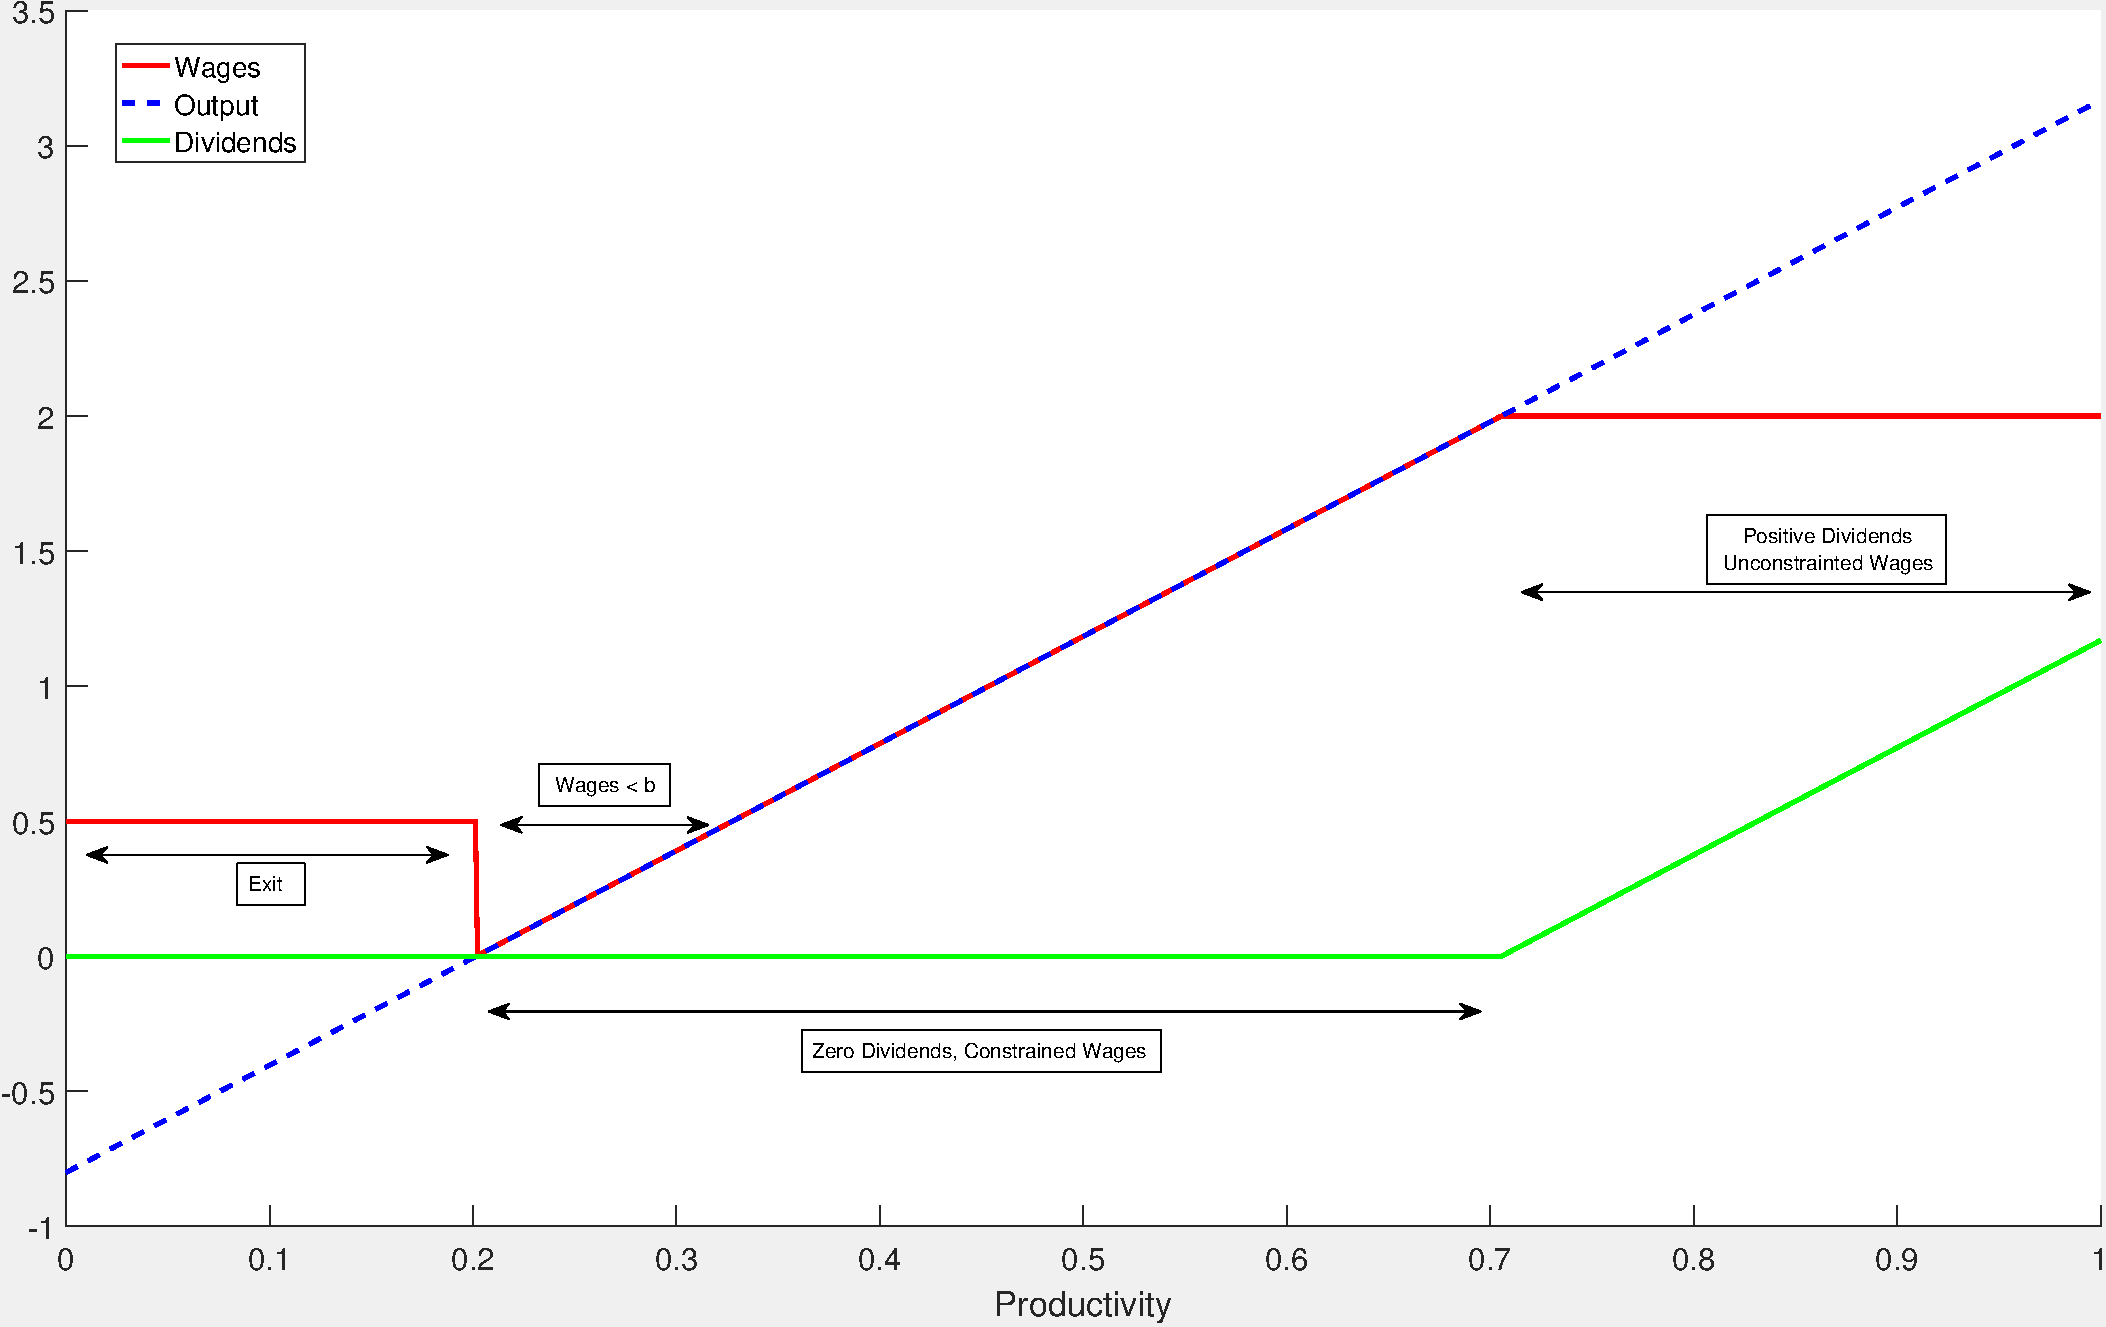
\includegraphics[scale=0.3]{figures/WagePeriod1}
	\label{fig:wageperiod1}
\end{figure}
}

\frame{\frametitle{Period 2 Wages}
	\begin{figure}
		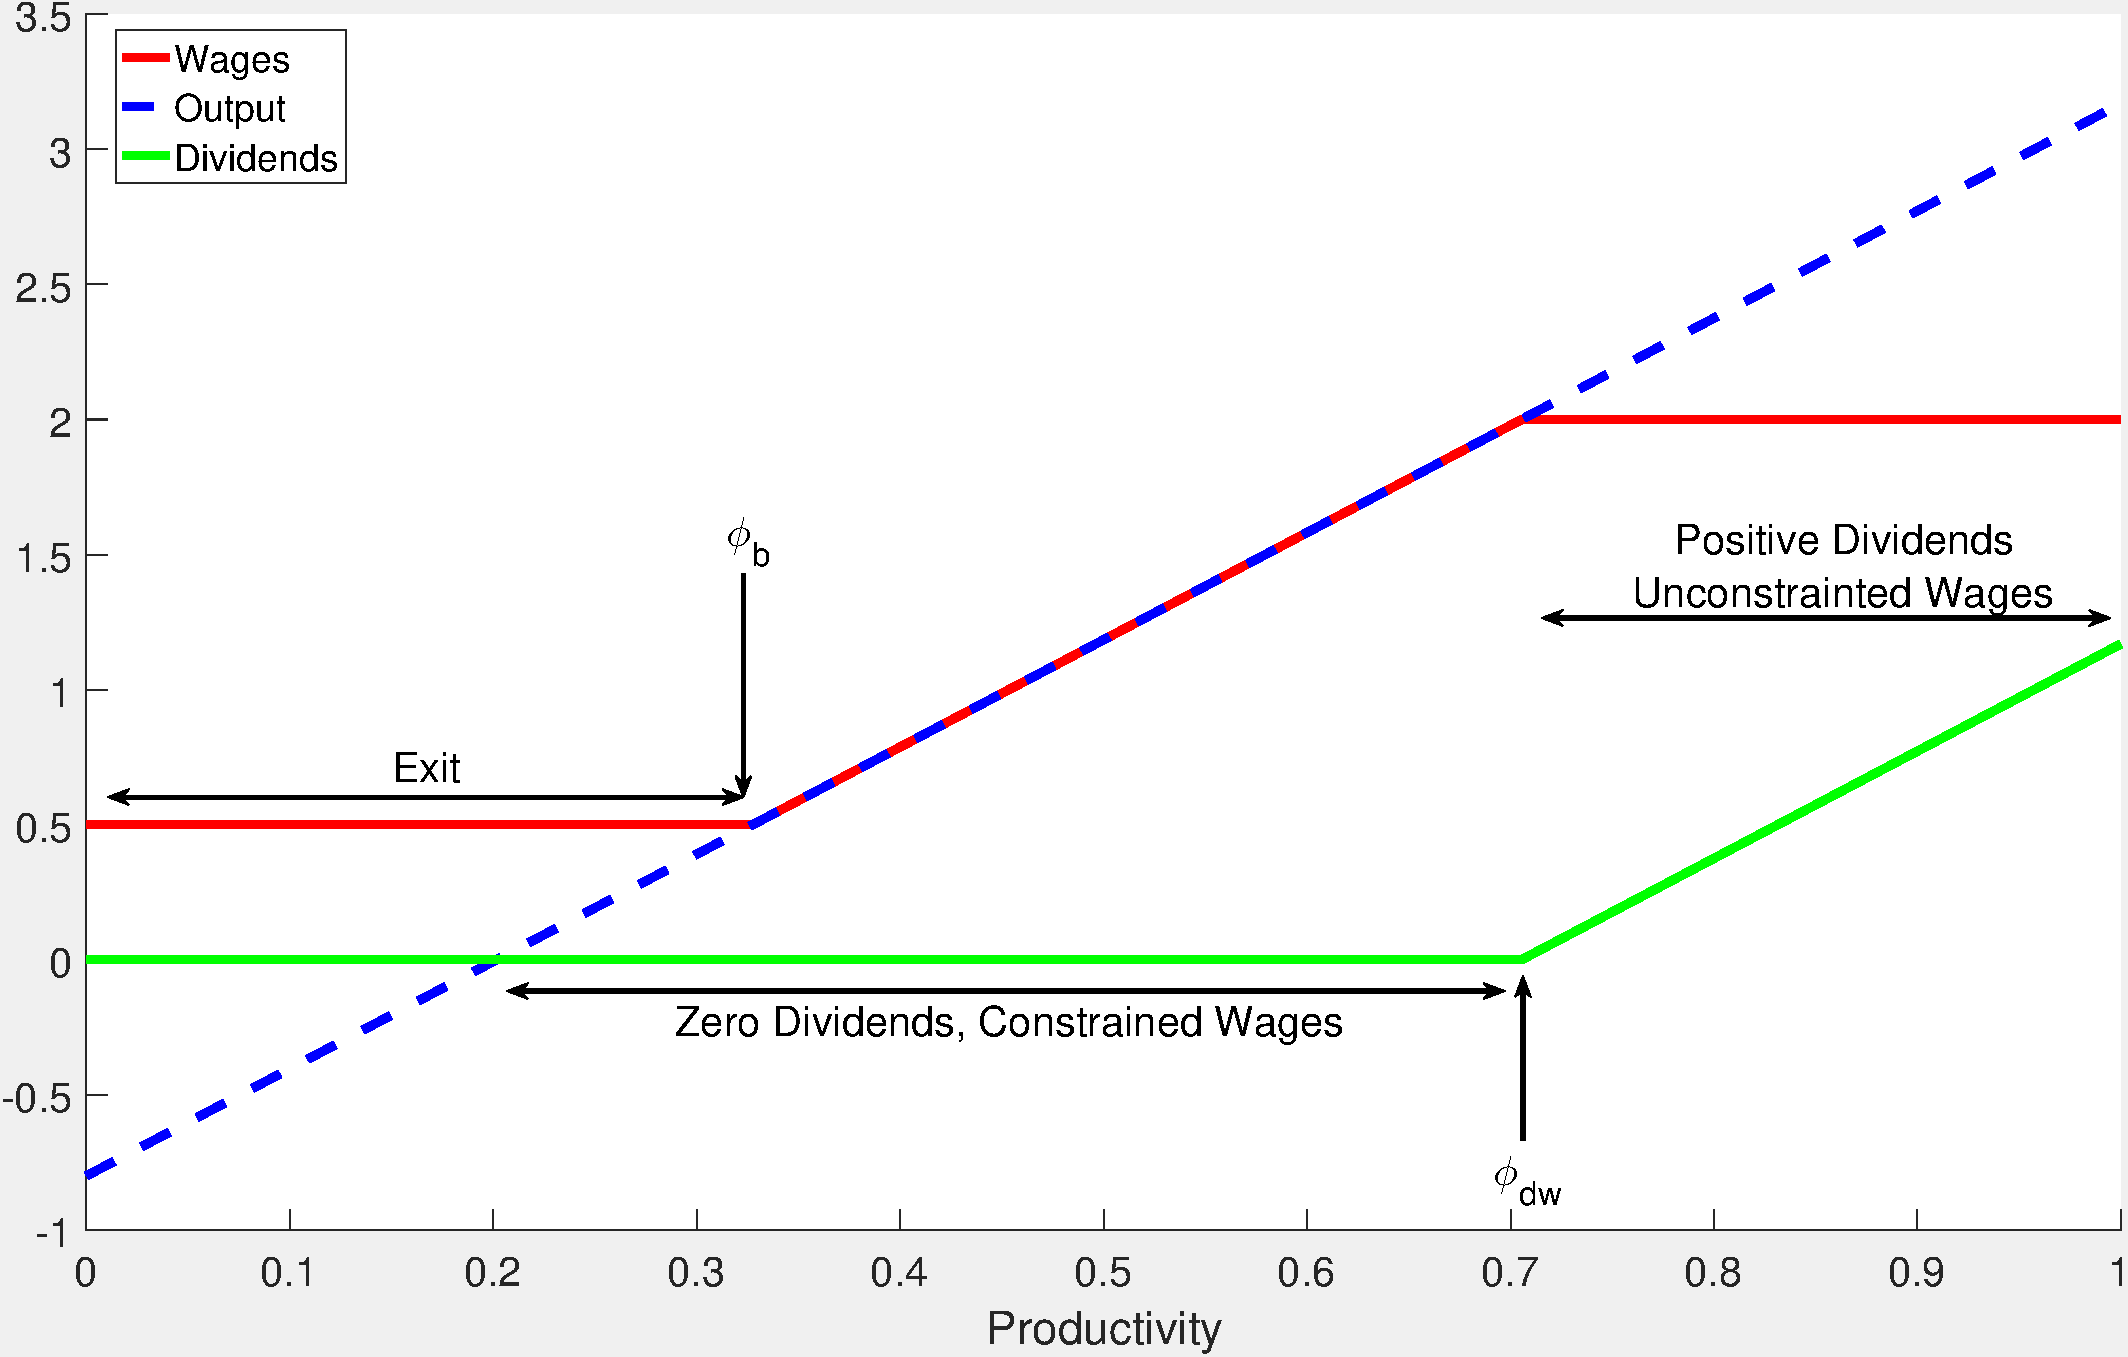
\includegraphics[scale=0.3]{figures/WagePeriod2}
		\label{fig:wageperiod1}
	\end{figure}
}




\frame{\frametitle{Worker's Problem}
	\begin{figure}
	\centering
	\begin{itemize}
		\item Firm's post \textit{unconstrained wage} contracts, $ \tilde{w} $
		\item \[U = \max_{\tilde{w}} p(\theta(\tilde{w})) \mathbb{E}\left(u_1(\tilde{w}) + \beta  u_2(\tilde{w})\right) \]
		\item 
	\end{itemize}
\end{figure}	
}

\frame{\frametitle{Dynamic Model with Labor Market Frictions}
	\begin{figure}
		\centering
		\begin{itemize}
			\item 
			\item
			\item
			\item
			\item
		\end{itemize}
	\end{figure}
}

\frame{\frametitle{Conclusion}
	\begin{figure}
		\centering
		\begin{itemize}
			\item 
			\item
			\item
			\item
			\item
		\end{itemize}
	\end{figure}
}

\end{document}
